\documentclass[12pt]{article}
\usepackage{amsfonts, epsfig}

\usepackage{graphicx}
\usepackage{fancyhdr}
\pagestyle{fancy}
\lfoot{\texttt{github.com/conorhoughton/COMS30127}}
\lhead{Computation Neuroscience - 6\_mp\_neurons (d) - Conor}
\rhead{\thepage}
\cfoot{}

\usepackage{graphicx}
\usepackage{pstricks}
\usepackage{listings}

\usepackage{tikz}

\usepackage{pgf}
\usepackage[utf8]{inputenc}
\usetikzlibrary{arrows,automata}
\usetikzlibrary{positioning}


\tikzset{
    neuron/.style={
           rectangle,
           rounded corners,
           draw=black, very thick,
           inner sep=2pt,
           text centered,
           },
}



\tikzset{
    area/.style={
           rectangle,
           draw=black, very thick,
           inner sep=2pt,
           text centered,
           },
}


\tikzset{
    gc/.style={
           rectangle,
           rounded corners,
           draw=red, very thick,
           inner sep=2pt,
           text centered,
           },
}


\tikzset{
    inh/.style={
           rectangle,
           rounded corners,
           draw=blue, very thick,
           inner sep=2pt,
           text centered,
           },
}



\tikzset{
    io/.style={
           rectangle,
           draw=green, very thick,
           inner sep=2pt,
           text centered,
           },
}



\begin{document}

\section*{McCulloch-Pitts neurons} 

The McCulloch Pitts neuron model, or Threshold Logic Unit, was
introduced in 1943 by Warren McCulloch and Walter Pitts as a
computational model of a neuronal network \cite{McCullochPitts1943}. Their thinking was that
neurons are joined to each other with connections of variable
strength; in the soma the inputs from other neurons are added up and
they determine the activity of the neuron in a non-linear way; they
also knew that neurons tend to ignore input up to some threshold value
before responding strongly. These properties they tried to include in
their model neurons.

Artificial neurons, of the sort used in artificial intelligence, are
described by a single dynamical variable, $x_i$ say for a neuron
labelled $i$; the value of $x_i$ is determined by the weighted input
from the other neurons:
\begin{equation}
x_i=\phi\left(\sum_j w_{ij} x_j-\theta_i\right)
\end{equation}
$\phi$ is an activation function, $\theta$ is a threshold and the
$w_{ij}$ are the connection strengths weighting the inputs from the
other neurons. The McCulloch Pitts neuron was the first example of an
artificial neuron and had a step function for $\phi$:
\begin{equation}
x_i=\left\{\begin{array}{ll}1&\sum_j w_{ij} x_j>\theta_i\\0&\mbox{otherwise}\end{array}\right.
\end{equation}
Thus, the neuron has two states, it is in the on state, $x_i=1$ if the
weighted input exceeds a threshold $\theta_i$ and an off state,
$x_i=-1$ if it doesn't; the picture you might have of how this
corresponds to the brain is that \lq{}on\rq{} corresponds to rapid
spiking and \lq{}off\rq{} to spiking at a much lower rate. The
$w_{ij}$, the connection strengths, are like the synapse strengths, a
positive $w_{ij}$ is an excitatory synapse and negative, an
inhibitory; a given neurons have have both negative and positive
out-going synapses, that is there is no restriction that says $w_{ij}$
always has the same sign for a given $j$, this is different from real
neurons where all the outgoing synapses from a given neuron are either
excitatory or inhibitory.

While it should be clear that this network has some of the properties,
very abstracted, of a neuronal network, it might not be so clear what
can be done with the neurons. When they were working, at the dawn of
the age of electronic computers, McCulloch and Pitts believed that
their neurons might form the natural unit in computer circuits, in
other words, they thought they might perform the role actually played
by logical circuits. In fact, it is still not clear if the artificial
neuron is or isn't the natural unit of computation in silicon since
they are a component in, for example, deep learning networks. In fact,
there are two major applications of McCulloch-Pitts neurons: the
perceptron and the Hopfield network; these two applications add a rule
for changing the connect strength to the original McCulloch-Pitts
neuron.

\subsubsection*{Perceptrons}

The perceptron is a machine that does supervised learning, that is, it
makes guesses, is told whether or not its guess is correct, and then
makes another guess. They were first discovered in 1957 by Frank
Rosenblatt \cite{Rosenblatt1958} and introduced to the world with great fanfare, it was
claimed that they would solve problems from object recognition to
consciousness: if you consider the perceptron as the forebearer of the
deep learning network, then perhaps we don't know if these claims will
be fulfilled, but we do know that the original perceptron proved quite
limited in artificial intelligence. It does, however, appear to
describe some neuronal processes, if we ignore the implementation
details.

Anyway, a percepton is made of two layers of neurons, an input layer
and an output layer of McCulloch-Pitts neurons. For simplicity lets
assume the output layer
has a single neuron. Now, if the input is given by
$\textbf{x}=(x_1,x_2,\ldots,x_n)$ the output, $y$, is
\begin{equation}
y=\phi(r)
\end{equation}
where
\begin{equation}
r=\sum_j w_j x_j-\theta
\end{equation}
and $\phi$ here is the simple Heaviside like activation function
described above. Now for a given input, if the actual value of the
output should be $d$ the error is $d-y$. The perceptron learning rule
is to change the $w_j$ weight by an amount proportional to the error
and how much $x_j$ was \lq{}to blame\rq{} for the error:
\begin{equation}
\delta w_j=\eta (d-y) x_j
\end{equation}
and
\begin{equation}
\delta \theta =  \eta (d-y)
\end{equation}
where $\eta$ is some small learning rate and
\begin{eqnarray}
w_j&\rightarrow& w_j+\delta w_j\cr
\theta&\rightarrow& \theta+\delta\theta
\end{eqnarray}
You can see how this might work, if $x_j$ was positive and $y$ was too
big, this would make $w_j$ smaller so in future $y$ would be smaller
when it had the same input. 

In fact, the perceptron can only solve problems with a linear
classifier: if we think of the $x_i$'s as parametrizing an
$n$-dimensional space then $\sum_iw_ix_i=\theta$ is a hyperplane in
that space, so a pattern $\textbf{x}$ is classified one way or the
other according to which side of that hyperplane it lies. Thus, the
perceptron works only if there is a hyperplane dividing the data into
two, with one class of data on one side and one on the other. In fact,
if the data is linearly separable the perceptron is guaranteed to
converge to a solution which manages this separation. Now, there will
not be a unique hyper-plane separating the two classes and the
perceptron won't, typically, find what you might regard as the
\lq{}best\rq{} hyperplane, where by best you might mean the line that
is, in some sense, as far from the individual data points as possible;
finding that best hyperplane is the idea behind the support vector
machine.

The perceptron learning rule can be motivated by thinking about error
minimization. Consider an error function
\begin{equation}
E=\langle(d^a-y^a)^2\rangle_a
\end{equation}
If $a$ labels lots of input, $\textbf{x}^a$, desired output $d^a$
pairs, with $y^a$ the actual output; the angle brackets are an average
over these pairs. Now consider the gradient of $E$ with $w_{i}$:
\begin{equation}
\frac{\partial E}{\partial w_{i}}=2\left\langle (d^a-y_a) \frac{\partial y^a}{\partial w_{i}}\right\rangle
\end{equation}
Now if we ignore for the moment the fact that the activiation function for the McCulloch-Pitt neuron isn't differentiable and write
\begin{equation}
y^=\phi(r)
\end{equation}
with 
\begin{equation}
r=\sum_{i}w_i x_i-\theta
\end{equation}
we have
\begin{equation}
\frac{dy^a}{dw_i}=\frac{d\phi}{dr}\frac{\partial r}{\partial w_i}
\end{equation}
so using
\begin{equation}
\frac{\partial r}{\partial w_i}=-x_i
\end{equation}
we get
\begin{equation}
\frac{\partial E}{\partial w_{i}}=-2\left\langle (d^a-y^a)x^a_i (\mbox{stuff involving the derivative of }\phi)\right\rangle
\end{equation}
Of course, in the McCulloch-Pitts case the \lq{}stuff involving the
derivative of $\phi$\rq{} is either zero or undefined, but we can that
this gives a similar learning rule: one way to reduce the error is to
move a tiny amount in the opposite direction to the gradient, the
gradient is the direction along which the value increases
quickest. The actual perceptron rule we gave updates a small bit after
every presentation rather than averaging first over a collection of
presentations, both approaches make sense. Here we have dealt with the
weights, the same approach can be applied to the threshold $\theta$.

This is the way to a more modern approach to the perceptron rule and
these days smooth, or mostly-smooth activation functions are used in
artificial neurons for this reason. The basic limitation of the
perceptron is that it has only one layer and so only learns a linear
classification; these days artificial neural networks have more than
one layer; this complicates the idea of adjusting the $w_i$ in a way
that is weighted by $x_i$, this, in a sense, changing the weight
according to how much it is \lq{}to blame\rq{} for the error. Back
propagation resolves this, it can be thought of as propagating the
error backwards from layer to layer; although another way to think of
it is as doing gradient descent on all the weights. At the moment the
back propagation algorithm is not considered very biological, though
it is very possible that when we understand why deep learning networks
are so effective it will be clear that the important aspects of the
algorithm can be recognized in neuronal dynamics.

\subsection*{The cerebellum as a perceptron}

The cerebellum has a number of striking features; it has a more
stereotypical structure than most brain area and this structure is
conaerved across species. It also has one of the brain's largest cells,
the Purkinje cell, and its most numerous, the granule cell.

\begin{figure}
\begin{center}
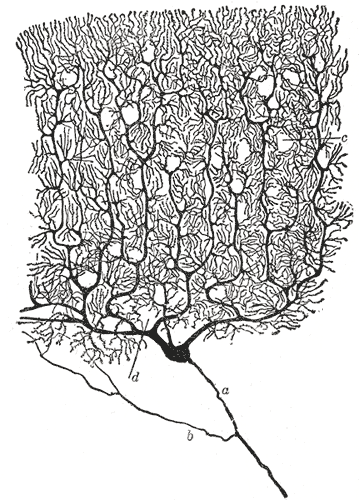
\includegraphics[width=7cm]{Purkinje_cell_by_Cajal.png}
\end{center}
\caption{A drawing by Santiago Ram\'{o}n y Cajal of a Purkinje cell. [Picture taken from \texttt{http://en.wikipedia.org/wiki/Golgi's\_method}]\label{fig:PC}}
\end{figure}

Purkinje cells have a distinctive structure with a huge, highly
branched, but flat dendritic arbor, see Fig.~\ref{fig:PC}; this allows
an extensive connectivity with each Purkinje cell receiving inputs
from around 100,000 other cells. In the cerebellum the Purkinje cell
are lined up like pages in a book, with their arbors lying in parallel
planes. They receive two excitatory inputs, weak inputs from parallel
fibres, axons that run perpendicular to the planes of the Purkinje
cell dendritic arbors, and a strong input from a climbing fibre, a
single axon which winds around the Purkinje cell and makes multiple
contacts with it, see Fig.~\ref{fig:cerebellum}.

\begin{figure}
\begin{center}
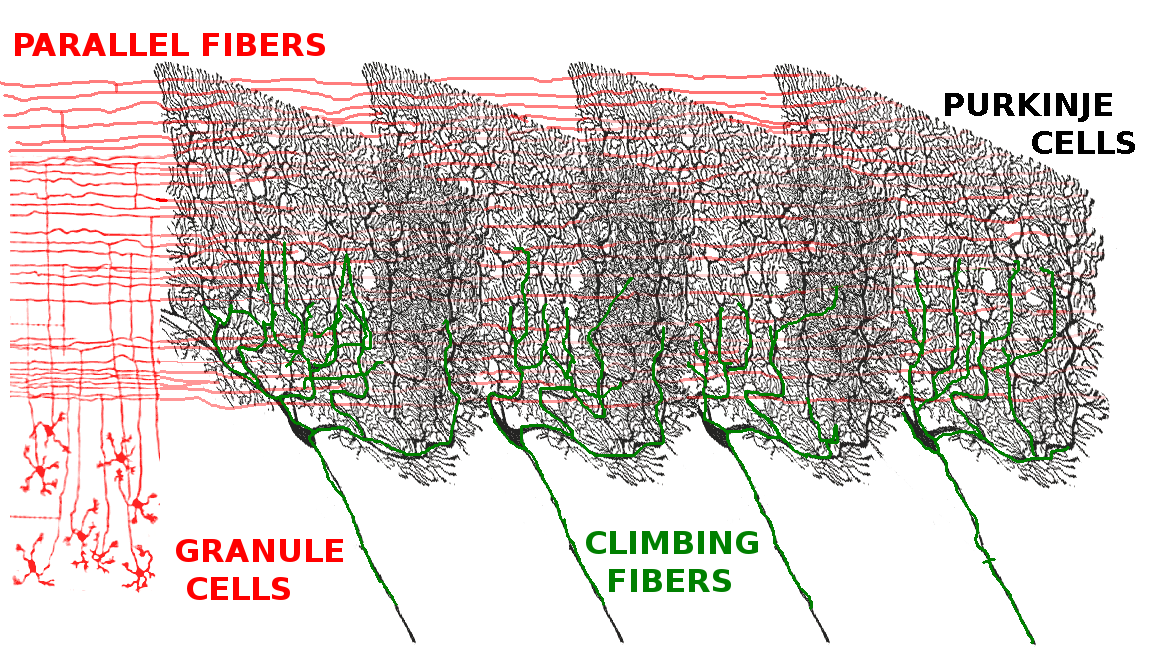
\includegraphics[width=11cm]{cerebellum.png}
\end{center}
\caption{A cartoon of the cerebellar circuitary. A vertical axon rises
  from each granule cells, splits once and then extends horizontally
  in two directions making connections with multiple Purkinje
  cells. Each Purkinje cell has its own climbing fiber which winds up
  around it.\label{fig:cerebellum}}
\end{figure}

\begin{figure}
\begin{center}
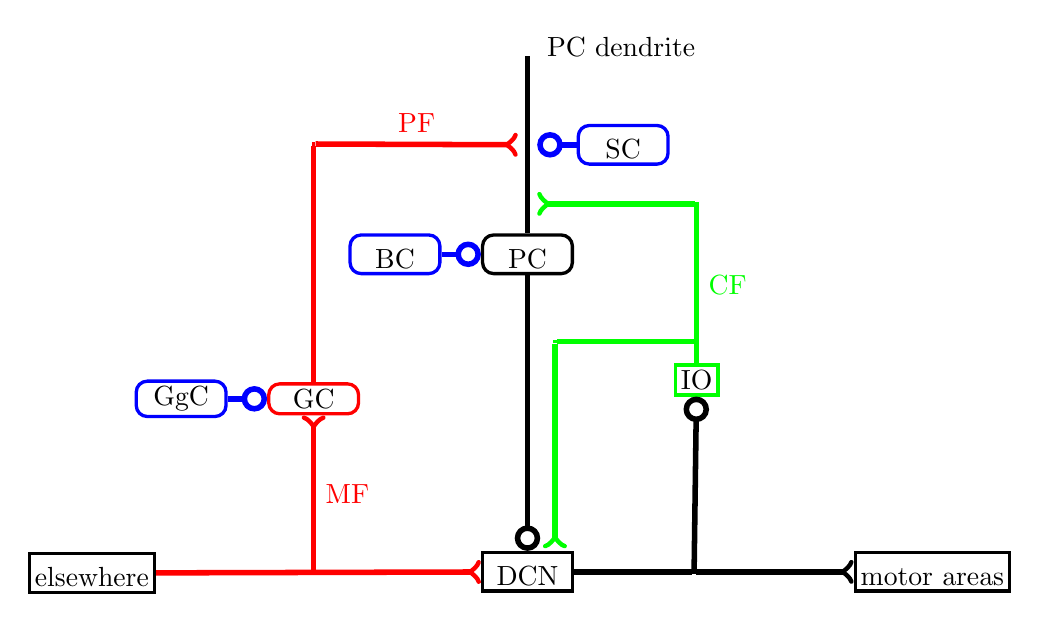
\begin{tikzpicture}
\node[neuron,text width=1cm, text height=0.35cm](PC){PC};
\node[inh,text width=1cm, text height=0.35cm,left = 0.5cm of PC](BC){BC};
\node[above = 1cm of PC](PCd){};
\node[inh,text width=1cm, text height=0.35cm,right = 0.5cm of PCd](SC){SC};
\node[above = 0.25cm of PC](PCc){};
\node[scale = 0.2,fill=green,right = 2cm of PCc](PCcr){};
\node[above = 1cm of PCd](PCdd){};
\node[right = 0cm of PCdd](){PC dendrite};
\node[left = 2cm of PC](PCl){};
\node[gc,text width=1cm,below = 1.5cm of PCl](GC){GC};
\node[inh,text width=1cm,left = 0.5cm of GC](GgC){GgC};
\node[scale = 0.2,fill=red,above = 3cm of GC](GCa){};
\node[scale = 0.01,fill=red,below = 2cm of GC](GCb){};
\node[io,below = 2cm of PCcr](IO){IO};
\node[scale =0.2,fill=green,above = 0.25cm of IO](IOa){};
\node[scale =0.2,fill=green,left = 1.75cm of IOa](IOl){};
\node[scale =0.01,below = 2.6cm of IOl](IOlb){};
\node[area,text width=1cm, text height=0.35cm,below  = 3.5cm of PC](DCN){DCN};
\node[scale=0.2,fill=black,right= 1.5cm of DCN](DCNr){};
\node[area,text height=0.35cm,right = 2cm of DCNr](ma){motor areas};
\node[area,text height=0.35cm,left = 2cm of GCb](ew){elsewhere};
\path (PCdd) edge[-,line width=2pt](PC);
\path (PC) edge[-o,line width=2pt] (DCN);
\path (IO) edge[-,green,line width=2pt] node[anchor=west]{CF} (PCcr);
\path (PCcr) edge[-<,green,line width=2pt] (PCc);
\path (GC) edge[-,red,line width=2pt] (GCa);
\path (GCa) edge[-<,red,line width=2pt] node[anchor=south]{PF}(PCd);
\path (GCb) edge[-<,red,line width=2pt] node[anchor=west]{MF} (GC);
\path (ew) edge[-<,red,line width=2pt] (DCN);
\path (DCN) edge[-,black,line width=2pt] (DCNr);
\path (DCNr) edge[-o,black,line width=2pt] (IO);
\path (DCNr) edge[-<,black,line width=2pt] (ma);
\path (IOa) edge[-,green,line width=2pt](IOl);
\path (IOl) edge[-<,green, line width=2pt](IOlb);
\path (GgC) edge[-o,blue, line width=2pt](GC);
\path (BC) edge[-o,blue, line width=2pt](PC);
\path (SC) edge[-o,blue, line width=2pt](PCd);
\end{tikzpicture}
\end{center}
\caption{A schematic of the cerebellar circuit. The granule cells (GC)
  receive input from a diverse range of other parts of the brain along
  the mossy fibers (MF). Each granule cell will combine input from
  just three or four mossy fibers and do this in lots of different
  combinations. The parallel fiber (PF) carries spikes from the GC to
  the Purkinje cell (PC) whose large dendrite is drawn as a line. The
  PC also receives input from a climbing fiber (CF) coming from
  Inferior Olivary Nucleus (IO). In turn it sends an inhibitory signal
  to the Deep Cerebellar Nucleus (DCN); the DCN has inhibitory neurons
  which act on IO and excitatory neurons which act on the motor
  system. The basket cells (BC), the Golgi cells (GgC) and the
  stellate cells (SC) are all local inhibitory
  cells.\label{fig:connectivity}}
\end{figure}

Another peculiarity is that the Purkinje cell has different responses
to different inputs; in response to multiple weak inputs from the
parallel fibers it fires a normal sort of spike, called in this
context a \textsl{simple spike}; in response to single spike from the
climbing fiber is fires a special spike, called a \textsl{complex
  spike}, with a leading spike, a number of small \lq{}spikelets\rq{}
and a sustained after-period of depolarization; this is illustrated in
Fig.~\ref{fig:spikes}.

\begin{figure}
\begin{center}
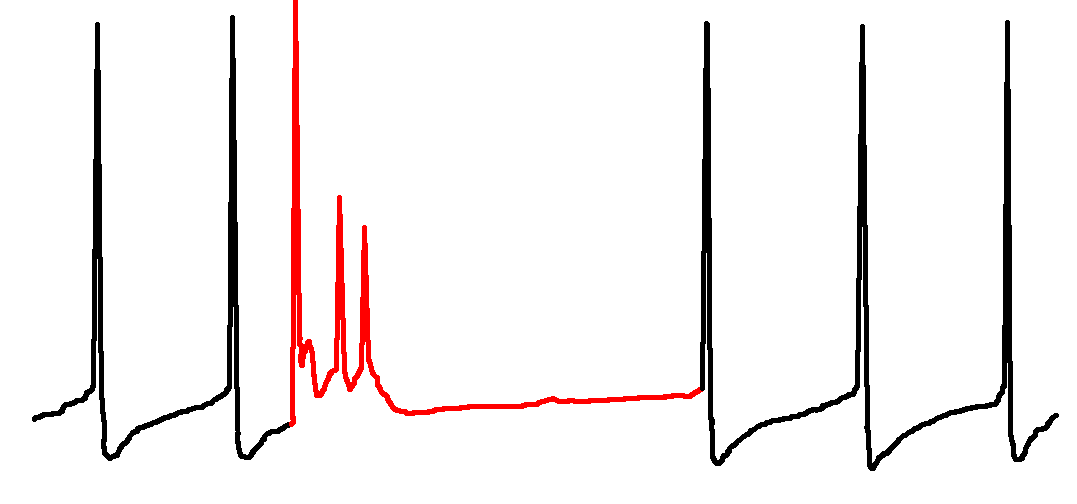
\includegraphics[width=8.cm]{complex_spike.png}
\end{center}
\caption{A complex spike. This drawing shows a simple spikes in black
  and a complex spike in red. The complex spike is followed by a long
  refractory period during which spiking is not possible. This is a
  sketch, not an actual recording, but a typical time scale would have
  this refractory period 50 ms long.\label{fig:spikes}}
\end{figure}

It is still unclear exactly what the cerebellum does; what is known is
that it is important for actions, fine motor control and
proprioception; problems with the cerebellum are associated with
ataxia, loss of fine motor control, poor motor learning and poor
balance. There is a specific gait associated with cerebellar damage,
one that exhibits a certain self-consciousness or vigilance is
required for movement. According to most ideas about cerebellar
function it is required for the calculation of fine motor signals
\cite{Albus1971a}, or for predicting the sensory or proprioceptive
consequences of motor actions \cite{GaoEtAl1996a}; it is believe it
encodes forward and backwards models of movement so that it predicts
the consequences of motor commands, or calculates the motor command
that will a particular movement.

Whatever exactly it does, it is widely believed, in accordance with
the Marr-Albus model \cite{Marr1969a,Albus1971a}, that the connections
from parallel fibers to Purkinje cells acts as a perceptron. Thus, if
$y$ is the output of the Purkinje cell and, in this simple model,
taking into account the fact Purkinje cells are inhibitory
\begin{equation}
y=-\sum{w_ix_i}
\end{equation}
where the $x_i$s are the activities in the parallel fibers and $w_i$
is the strength of the synapse from the $i$th parallel fiber to the
Purkinje cell. The idea in the Marr-Albus model is that the climbing
fiber carries the error signal $d-y$ making the cerebellum an example
of supervised learning.

\subsection*{Hopfield network}

In contrast to a perceptron, a Hopfield network is a recurrently
connected network; it is intended to perform pattern completion and
was proposed by John Hopfield in 1982 \cite{Hopfield1982}, though other people had had the
idea before in different contexts. The idea behind a Hopfield network
is that you evolve the network according to the McCulloch-Pitts
relation, so, in the synchronous update version, from one iteration to
the next
\begin{equation}
\hat{x}_i=\phi\left(\sum_j w_{ij} x_j\right)
\end{equation}
and then $x_i\rightarrow \hat{x}$; that is all the nodes update using
the old values. In the most common version of a Hopfield network, the $w_{ij}$ are symmetric, that is
\begin{equation}
w_{ij}=w_{ji}
\end{equation}
The threshold values $\theta_i$ have been set to zero, this is
something you can do in a Hopfield network. In the asynchronous
scheme, the you update the nodes one-by-one, for example, after
choosing a random node.

Now, there is an \lq{}energy\rq{} associated with a Hopfield network:
\begin{equation}
E=-\frac{1}{2}\sum_{ij} w_{ij}x_ix_j
\end{equation}
and you can show than if you update a node you will reduce the energy;
roughly speaking if you update a node $x_i$ then it is more likely to
have the same sign as a connected node $x_j$ if the connection between
them is large and positive and an opposite sign if the connect is
large and negative. It can be shown that update the nodes will evolve
the system to a local minimum.

Now the question is how to create the local minima? Two versions:
\begin{equation}
w_{ij}=\frac{1}{N}\sum_a x^a_ix^a_j
\end{equation}
or 
\begin{equation}
\delta w_{ij}=\eta (x_i-\alpha)(x_j-\alpha)
\end{equation}
where $N$ is the number of patterns to be stored, and $a$ indexes the
patterns.


\begin{thebibliography}{10}

\bibitem{McCullochPitts1943}
McCulloch, W and Pitts, W. (1943). A logical calculus of the ideas immanent in nervous activity. 
\newblock Bulletin of Mathematical Biophysics, 5:115--133. 

\bibitem{Rosenblatt1958}
Rosenblatt, F. (1958), The Perceptron: A Probabilistic Model for Information Storage and Organization in the Brain, Cornell Aeronautical Laboratory.
\newblock Psychological Review, 65:386--408.

\bibitem{Albus1971a}
Albus, JS. (1971) A theory of cerebellar function. 
\newblock Mathematical Biosciences 10: 25--61.


\bibitem{GaoEtAl1996a}
Gao J-H, Parsons LM, Bower JM, Xiong J, Li J and Fox PT (1996) Cerebellum implicated in sensory acquisition and discrimination rather than motor control.
\newblock Science 272: 545--7. 

\bibitem{Marr1969a}
Marr, D (1969) A theory of cerebellar cortex.
\newblock Journal of Physiology 202: 437--70.

\bibitem{Hopfield1982}
Hopfield, JJ. (1982) Neural networks and physical systems with emergent collective computational abilities.
\newblock Proceedings of the National Academy of Sciences of the USA, 79:2554--2558.


\end{thebibliography}

\end{document}

